% !TEX encoding = Mac Central European Roman
\documentclass[a4paper,12pt]{article}

\usepackage{amsmath, amssymb, mathtools, verbatim, bm, xcolor, hyperref}
%\usepackage[polish]{babel}
\usepackage{polski}
\usepackage[T1]{fontenc}
\usepackage[utf8]{inputenc}
\usepackage{textcomp}
%\usepackage[macce]{inputenc}
%\usepackage[latin2]{inputenc}
\usepackage{physics}
\usepackage[textsize=tiny]{todonotes}
\definecolor{lightgray}{gray}{0.90}
\newtheorem{theorem}{Theorem}
\usepackage{framed}
\renewenvironment{leftbar}[1][\hsize]
{% 
\def\FrameCommand 
{%

    {\hspace{-3pt}\color{black}\vrule width 3pt}%
    \hspace{0pt}%must no space.
    \fboxsep=\FrameSep\colorbox{lightgray}%
}%
\MakeFramed{\hsize#1\advance\hsize-\width\FrameRestore}%
}
{\endMakeFramed}
\setlength{\FrameSep}{0pt}

%\usepackage{showframe}
\usepackage[left=70pt,
			right=70pt,
            top=50pt,
%            textwidth=345pt,
            marginparsep=0pt,
            marginparwidth=70pt,
%            textheight=692pt,
%            footskip=50pt
            ]
           {geometry}
%\textwidth=16.5 truecm
%\textheight=25 truecm
%\hoffset=-2.5 truecm
%\voffset=-2 truecm

\def\baselinestretch{1.2}

%\pagestyle{empty}

\begin{document}

\title{Non-equilibrium systems and growth of complexity}

\author{Michał Mandrysz \\
Instytut Fizyki, Uniwersytet Jagielloński, \\ul. Łojasiewicza
11, 30-348 Kraków, Polska }



\maketitle

\tableofcontents

\section{Historical introduction}

\subsection{Summary of Schr{\" o}dinger{'}s contributions}

By writing his book {``}What is life?{''} (1944) Schr{\" o}dinger inspired generations of physicists to answer the alluring (though not easy) question
of the role of physics in biological processes. In any event it probably wouldn't be an exaggeration to say that Schr{\" o}dinger himself (as he
admits), was inspired by the work of German-American physicists Max Delbr{\" u}ck; who helped launch the molecular biology research program in the
late 1930s and explained (in main part) the mechanism of heredity and mutation.

Regardless, Schr{\" o}dinger makes some very essential observations on the nature of living organisms which I shall describe here shortly.

First, their operation (living organisms) as a macroscopic system resembles approximately, a purely mechanical system rather than a thermodynamical
system. Even though their size is far from what is considered a thermodynamic limit, they tend stay unaffected (in special environments) by random
molecular motion known as heat and; at the same time, evade the decay towards equilibrium for an unusually long time. This is essentially the definition
of a living system.

Secondly, he notices that the way an organism accomplishes the above is through the exchange of energy and matter with it's environment, that leaves
it's own internal state in low entropy. He withdraws from considerations of free energy, although he acknowledges that the exact physical understanding
should be accomplished through it rather than through entropy. Worth mentioning is his hypothesis of {``}life intensity{''} the term which ought
to parallel with the rate at which the system produces entropy.

Thirdly, each cell depends on very small group of atoms, the genetic code, which determine it's evolution, something unprecedented, beyond the description
of ordinary statistical physics. Perhaps, a partial explanation for this dynamical behavior (rather than statistical) can be traced to rigidity and
tightness of chemical bonds. However the very vital point Schr{\" o}dinger tries to make is the hypothesis, that there must exist a yet unknown,
new law of physics that would explain fully how order can be produced out of order. The formulation of this law is to my knowledge; still in development.

Lastly, even though Schr{\" o}dinger introduces some quantum mechanics principles, like the uniqueness of Heitler-London bond in order to defend
the theory laid down by Delbr{\" u}ck, he assures that quantum indeterminacy should play only marginal role in the future laws of dynamics of living
systems.

\subsection{Summary of Prigogine contributions}

The term {``}dissipative structures{''} was first used by Ilya Prigogine (http://bactra.org/notebooks/dissipative-structures.html) and although Prigogine ideas were not really correct ones it might be worth to recall some of them.

\subsection*{Nobel Lecture (8 December 1977)}

Prigogine nobel prize lecture {``}Time, structure and fluctuations{''} begins with the critique of Helmholtz free energy and the assertion that living
system posses a different type of functional order which can be traced to their non$--$equilibrium state. This statement is consistent with the today{'}s predominant view.

{``}However thermodynamic potentials exist only for exceptional situations{''}

One of his often cited contributions is connected with a term for entropy for open systems, an extension of Clausius entropy for isolated systems:

\begin{displaymath}
	dS=d_iS+d_eS
\end{displaymath}


Where \(d_iS\) is connected with entropy produced within the system and \(d_eS\) is the entropy transferred across the boundaries of the system.
The second law states that \(d_iS\geq 0\), so if a system is to stay in law entropy state it{'}s production must be compensated by an inflow of negative
entropy.

He then develops an explicit expression for entropy production, assuming that even outside equilibrium (but near) entropy depends only on the same
variables as at equilibrium ({``}local{''} equilibrium)

\begin{displaymath}
	P=\frac{d_iS}{dt}=\sum _{\rho } J_{\rho }X_{\rho }\geq 0
\end{displaymath}


where \(J_{\rho }\) are the rates of the various irreversible processes involved (chemical reactions, heat flow, diffusion$\ldots $) and \(X_{\rho
}\) are the corresponding, generalized forces (affinities, gradients of temperature, of chemical potentials$\ldots $). The flows are described using
different empirical laws (Fourier{'}s law, Fick{'}s law, etc.) 

\begin{displaymath}
	J_{\rho }=\sum _{\rho } L_{\rho \rho '}X_{\rho '}
\end{displaymath}


Onsager relations \(L_{\rho \rho '}=L_{\rho '\rho }\)

Prigogine rightly criticized the efforts to extend the principle of minimum entropy production (which is valid only very near equilibrium)
to non-equilibrium regimes, showing that. What exactly is this principle is well explained by Prigogine; when a system is constricted by a boundary
condition and perturbed, the entropy production will increase, but then the system settles down to the state of {``}least dissipation{''}.\\
An example of a process such process, namely Rayleigh$--$B{\' e}nard convection is given, which he perceives as a prime example of occurrence of
{``}dissipative structures{''} which fail to be described by Boltzmann laws. In Prigogine view the fluctuations are the trigger for the instabilities
instabilities, which in turn give rise to spacetime structure. Here instabilities carry the sense of bifurcations of equations of motion.

[I need to learn more about Nicolis work on dynamics of chemical reactions]

Furthermore Prigogine develops an uncommon perspective on the microscopic equations of motion, which in his opinion should not be invariant under
time inversion.\\
A proposed way to achieve this is through a non$--$unitary transformation which yield a type Lyapounov function, analogue to Bolzmann H-function.
The goal was to obtain a microscopic representation of entropy. It{'}s known in literature as Misra-Prigogine-Courbage theory of irreversibility.

Prigogine view on reversibility are probably best summarized by the quotes {``}I have always found it difficult to accept this conclusion [macroscopic
irreversibility emerging from initial conditions] { }especially because of the constructive role of irreversible processes. Can dissipative structures
be the result of mistakes?{''}

[At the present moment I can{'}t comment much on this, but some extensive critique can be found {``}Science of Chaos or Chaos in Science{''} by Bricmont]

The best account (or the most understandable) of Prigogine views are perhaps his own words in {``}Laws of Chaos{''} - {``}The essential condition
is that the microscopic description of the universe be made in terms of unstable dynamical systems. This is a radical change in point of view. From
the point of view of classical physics, stable systems were the rule and unstable systems the exceptions. We are now reversing that perspective.{''}\\
First it{'}s not true that stable systems are the rule in classical physics, one can easily devise classical examples of unstable systems following
purely classical mechanics, the reason why they are not being analyzed is that analytic methods fail to solve them. Prigogine seems to require more
complexity to explain complexity, which is in my opinion not needed.

\section{Entropy in quantum systems}
\subsection{von Neumann entropy}

Although this work is meant to stay within the classical limit, it might be worth while to clear out the notion of entropy in quantum context.

The von Neumann entropy is defined as 

\begin{equation}
  S_{vN}= -\Tr(\hat{\rho} \log{\hat{\rho}}).
\end{equation}

For which the general form of the density matrix operator is

\begin{equation}
	\hat{\rho}=\sum_k p_k \ket{\psi_k}\bra{\psi_k} 
\end{equation}

in case of pure state $\ket{\psi}$ the density matrix is simply
\begin{equation}
  \hat{\rho} = \ket{\psi}\bra{\psi}
\end{equation}

and it is easy to verify that the entropy of a pure state is equal to zero. The entropy of mixed state is always greater than zero.
If the system is in a pure state, it will continue to be in a pure state as long as it stays isolated. For a mixed state, the degree of mixedness measured by the entropy will stay constant as long as it is isolated. This follows from the fact that the time evolution is unitary and the eigenvalues of the density operator therefore do not change with time.

An interesting question one might ask (and not really discussed in textbooks) is how the entropy changes after a measurement of a particle in many-body system which, initially, was in pure state.

Without loss of generalization let's consider an isolated system of two identical particles described solely by their momentum states.
In the scenario of two particles of identical momentum we can write the initial pure state as 
\begin{equation}
  \ket{2,0,0,...}
\end{equation}
which entropy is of course zero.  
In second quantization formalism the measurement of a particle is realized by the field operator $ \hat{\Psi}(x) =\sum_k \phi_k(x)\hat{a}_n$ which annihilates a single particle at position $x$.
Therefore after the measurement of particle at some position $x$, one particle is "virtually" removed from the system under consideration, but the system stays in pure state
\begin{equation}
  \hat{\Psi}(x)\ket{2,0,0,...}=\phi_1(x)\ket{1,0,0,...},
\end{equation}
which entropy is zero. It's important to notice though that our system lost a particle and therefore the systems before and after measurement are not equivalent! Of course, in reality the particle doesn't disappear. After determination of it's position by experiment ($\Delta x \to 0$), the uncertainty of it's momentum approaches infinity ($\Delta p \to \infty$), which means that we can reconstruct the state using a linear combination of states with \textit{any} value of momentum:

\begin{equation}
  c_1\ \ket{2,,0,...}+c_2\ \ket{1,1,0,...}+  c_3\ \ket{1,0,1,...}+...
\end{equation}
where the  squared modulus of the coefficients has to sum up to one ($ \sum_i \left| c_i \right|^2 = 1 $).

Now depending on the precision of the measurement we can recalculate entropy of course getting a value greater than zero. If we would perform the same analysis for a pure state of two particles in different states i.e. $ket{1,1,...}$ then we would obtain an increase of entropy even without accounting for the lost particle.
\todo{Correct also for correlated systems?}
This crude example gives a clear illustration of the fact that after \textbf{any} measurement the von Neumann entropy has to increase. However it's change is ultimately related to lost information about the system in the act of the measurement.

There's another interesting feature of quantum entropy, namely inequalities that it fullfills.
If we bipartite the system into subsystems $A$ and $B$ each containing it's own set of commuting observables, then in order to calculate the entropy $S_A$ of a subsystem $A$ we need to calculate the entropy with respect to density matrix traced over the other subsystem, namely
\begin{equation}
  \hat{\rho}^A = \Tr_B \hat{\rho} 
\end{equation}
then in general the following identities are satisfied

\begin{equation}
\begin{aligned}
	S(\rho) &\leq S_A + S_B	\\
	S(\rho) &\geq \left| S_A - S_B \right|
\end{aligned}
\end{equation}

The interpretation of the first inequality is that the full information about the states of the subsystems $A$ and $B$ will in general not be sufficient to give full information about the state of the total system $A+B$. When there are correlations between the two subsystems, these are not seen in the description of $A$ and $B$ separately.

\section{Departure from equilibrium}

Almost a hundred fifty years (1870s) have passed since Ludwig Boltzmann proposed his statistical interpretation of entropy, which back then created a heated debate among prominent physicists of that time. 
One of the opposing arguments known as the Loschmidt paradox, has been understood long ago to be no threat to the Second Law of Thermodynamics. However the formal argument defending the Second Law appeared as late as in 1993, under the name of The Fluctuation Theorem discovered by Evans at al.

This example demonstrates the enormous difficulties connected with justification of (equilibrium) physical intuitions into firm mathematical formalism which in fact required the departure into non-equilibrium statistical mechanics.

[...]

Systems out of equilibrium can exhibit a variety of behaviours including relaxation, ageing, various meta-stable states, and steady states.
Even at steady state the difficulties seem to pile up as the basic state functions, such as temperature or entropy cease to exist outside of near equilibrium and the distribution functions appear fractal and non-analytic \cite{Dewar:2014ek}.

Even though the descriptions of non-equilibrium phenomena are most often being associated with names of Prigogine or Schr{\" o}dinger which undeniably have had an enormous influence on the field in question, they were not however the first.
The earliest efforts into explaining (near) non-equilibrium behaviour in a systematic way can be traced back to Einstein and theory of fluctuations [...] then to Lars Onsager's reciprocal relations


In 1993 Evans et al discovered a relation known as the Fluctuation Theorem (FT), which gives an analytical expression for the probability of observing Second Law violating dynamical fluctuations in thermostatted dissipative non-equilibrium systems.
The Fluctuation Theorem does much more than merely prove that in large systems observed for long periods of time, the Second Law is overwhelmingly likely to be valid. The Fluctuation Theorem quantifies the probability of observing violations of the Second Law in small systems observed for a short period of time \cite{Evans:2002gy}. The quantitative predictions made by the fluctuation theorem have been confirmed experimentally, both using laboratory experiments and using molecular dynamics computer simulations.

%TODO: Incorporate the following into bulk text
The frontier of non-equilibrium physics is being pushed forward by many groups and the specifics of their approaches differs. 
In classical physics part, the stochastic approach pioneered by Christopher Jarzynski and Gavin Crooks focuses on derivation of practical theorems and their numerical side. In fact the derivation of the fluctuation theorem by Crooks, although very lucid, depends on specific definitions of heat and work. One could argue for a more general approach and this is exactly what the Australian group of Evans et al. does. They start from the perspective of phase space evolution and first introduce the concept of dissipation, arguing why the concept of entropy production doesn't suffice and pointing out weaknesses of classical statistical mechanics constructs for description of non-equilibrium phenomena. Building on careful and general definitions they arrive at theorems of Crooks and Jarzynski. In this work we'll perform a continuous connection of the two approaches leading to a complete overview of the topic.

On quantum side,... 
%TODO: Finish the quantum side
\subsection{Gibbs entropy}

In comparison to Boltzmann entropy, Gibbs entropy is well defined also for a system of interacting particles.


%TODO: Add Jaynes - Gibbs vs Boltzmann Entropies

In Hamiltonian systems Gibbs entropy stays constant.
The constancy of entropy in Hamiltonian systems was first discovered by Gibbs in 1903 and was commented on extensively but inconclusively by Ehrenfest review of the foundations of statistical mechanics.

That however doesn't mean that the concept of Gibbs entropy 
is useless.

%TODO: Proof from page 43

\subsubsection{Simple model}
Let's consider a model consisting of three elements: the cooler $C$, the heater $H$ and the system under consideration $S$, staying out of equilibrium.
We assume, that the temperatures of the cooler and the heater stay constant, and that heat $Q_H$ flows into the system $S$ and heat $Q_C$ flows out. The situation is illustrated by the picture \ref{Fig2}.
\begin{figure}[ht!]
\centering 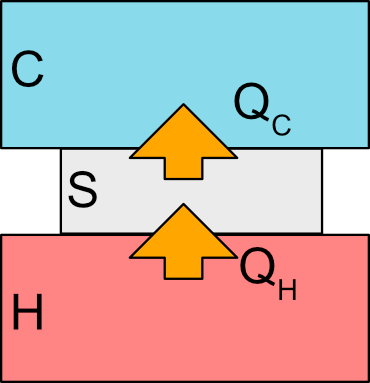
\includegraphics[width=6cm]{system} \caption{System (S) model}
\label{Fig2} 
\end{figure}

Treating the heater and the cooler as the environment, we can think of our system $S$ as an open system.
Further on we'll analyze the system $S$ from the perspective of internal $(i)$ entropy production
and external $(e)$ entropy flux, flowing \emph{to} the system $S$. 
Of course the change in entropy will be the sum of those two contributions:
\begin{equation}
dS_S=dS_i+dS_e.
\label{entrosum}
\end{equation}

In the current analysis let's consider a situation in which the same amount of heat flows in as flows out, that is $dQ_C=-dQ_H$. Using this relation we get the following term for the change of entropy:
\begin{equation}
dS_e=\frac{dQ_H}{T_H}+\frac{dQ_C}{T_C}=dQ_H\left(\frac{1}{T_H}-\frac{1}{T_C}\right)
=dQ_H\left(\frac{T_C-T_H}{T_HT_C}\right)<0.
\label{dSe1}
\end{equation}
From which it follows, that the heat flow takes the entropy out of our system.
For the purpose of further discussion we introduce the concept of rate of entropy change connected with the heat flow:
\begin{equation}
j_e \equiv  \frac{dS_e}{dt}. 
\end{equation}
In the considered scenerio, the $j_e$ is held constant (steady-state) and we suspect a continuous fall in system's entropy

Yet, moving away from the equilibrium state we suspect, that the a major role will be played by $dS_i$ moving the system back to equilibrium state. Similarly, as before we define the rate of internal entropy production:

\begin{equation}
j_i \equiv \frac{dS_i}{dt}.   
\end{equation} 

When $T_H=T_C$, i.e. the system is in equilibrium with constant entropy $S_{EQ}$ then it follows that $j_i=0$.
Therefore the rate of internal entropy production $j_i$ should be a function  of system's entropy $S_S$, i.e. $j_i = j_i(S_S)$ with the boundary condition $j_i(S_S=S_{EQ})=0$. 

Near the equilibrium state $S_S=S_{EQ}$, we can Taylor expand the function $j_i(S_S)$ to it's linear term
\begin{equation}
j_i(S_S)=j_i\left(S_{EQ}\right)+\left(S_S-S_{EQ}\right)C_1+\mathcal{O}\left(S_S^2\right),
\end{equation} 
fulfilling $j_i\left(S_{EQ}\right)=0$. 

The dimensional and stability analysis tells us that $C_1$ has the dimension of inverse time and in the case of 
$j_e=0$ should simply be equal to $S_{EQ}$, therefore:

Using the equation (\ref{entrosum}) we get
\begin{equation}
\frac{dS_S}{dt}=j_i\left(S_S\right)=\left(S_S-S_{EQ}\right)C_1, 
\label{stab}
\end{equation} 
Now we set $C_1 = -\frac{1}{\tau}$, where $\tau$ is a positive defined relaxation constant.

The solution of the equation (\ref{stab}) is then
\begin{equation}
S_S(t) =S_{EQ}+(S_0-S_{EQ})e^{-t/\tau}, 
\end{equation}
where the initial condition was set $S_S(0)=S_0$.


Now we include the term $j_e$ into our considerations.
In this case the equation (\ref{entrosum}) results in the following 
\begin{equation}
\frac{dS_S}{dt}=j_e + j_i\left(S_S\right)=j_e +\frac{S_{EQ}-S_S}{\tau}.
\label{dSSdt}
\end{equation} 

 
Given a boundary condition $S_S(0) =S_{EQ}$ it has a solution
\begin{equation}
S_S(t)=S_{EQ}+j_e\tau \left(1-e^{-t/\tau }\right),
\end{equation} 
where $j_e$ is a negative constant (graph of this function is presented on \ref{Fig4}). 
In the limit $t\rightarrow \infty$ the entropy of the system falls to the minimal value
\begin{equation}
S_{min}=S(t\rightarrow \infty) =S_{EQ}+j_e \tau < S_{EQ}.
\end{equation}

\begin{figure}[ht!]
\centering 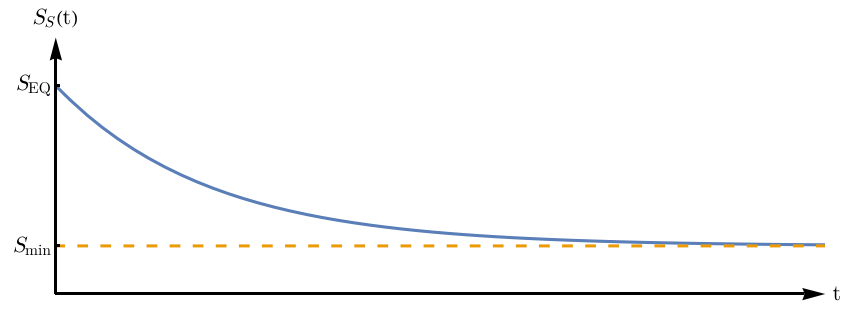
\includegraphics[width=12cm]{wykres3} 
\caption{Inducing lower entropy with heat flow.}
\label{Fig4} 
\end{figure}

This is of course consistent with the second law of thermodynamics as we're describing an open system.
It's easy to notice that the total entropy change is equal to $dS=dS_i \geq 0$ (for simplicity it was assumed that the heater and cooler don't act as producers of entropy).




\subsection{MaxEnt}

The essence of MaxEnt method can be summarized in the formula for maximization of relative entropy (negative Kullback-Leibler divergence)

\begin{displaymath}
  H(p\lor q) = -\sum_i \ln p_i \frac{p_i}{q_i}
\end{displaymath}
with respect to $p_i$ (new aposteriori distribution). $H(p||q)$ can be interpreted as the information gained by using $p_i$ instead of $q_i$.


\subsection{Near equilibrium results and concepts}

\subsubsection{Theory of Fluctuations}

Let us consider an adiabatically insulated system and a number of variables $x^i (i=1,...,n)$ which in the equilibrium state assume values $ x_0^i $, we can account for small variations ($\alpha^i$) by setting

\begin{displaymath}
  x^i = x_0^i + \alpha^i.
\end{displaymath}

The entropy in a state differing from the equilibrium state will be $S=S_0+\Delta S$, where $\Delta S$ is of the form

\begin{displaymath}
  \Delta S = - \frac{1}{2} \sum_{i,k} S_{ik} \alpha^i \alpha^k
\end{displaymath}
where $ S_{ik} $ is a positive definite form. The probability distribution for the $\alpha^i$ is given by

\begin{displaymath}
  W(\alpha^1,...,\alpha^n)d\alpha^1 ... d\alpha^1= \frac{e^{k_B \Delta S} d\alpha^1...d\alpha^n}{\int ... \int e^{k_B \Delta S} d\alpha^1...d\alpha^n}
\end{displaymath}

where $k_B$ is Boltzmann's constant.

Define

\begin{equation}
\gamma_i =\sum_k S_{ik} \alpha^k; \label{gammai}	
\end{equation}
  

then it is easily shown that

\begin{equation}
\langle \gamma_i \alpha^l \rangle = k_B \delta_i^l	
\end{equation}

Assuming ergodicity, this average may be interpreted either as an average over a microcanonical ensemble of systems, or as a time average for one single system.
By solving eq. \ref{gammai} for $\alpha^i $ we get

\begin{equation}
  \alpha^i=\sum_l S^{il}\gamma_l,
\end{equation}
and thus we find

\begin{equation}
	\langle \alpha^i \alpha^j \rangle = k_B S^{ij}   
\end{equation}

Let's suppose that $\alpha^i$ are even functions of the particle velocities with respect to time reversal.
The fact that its average future behaviour is identical to it's average past behaviour can be expressed by the equation:

\begin{equation}
  \langle \alpha^k (t+\tau)_{\alpha^{i \neq k}} \rangle =   \langle \alpha^k(t-\tau)_{\alpha^{i \neq k}} \rangle
\end{equation}

where the suffixes denote the values that remain fixed. Multiplying by $\alpha^l(t)$ and taking the average, we find

\begin{equation}
  \langle \alpha^l(t) \alpha^k (t+\tau) \rangle = \langle \alpha^l(t) \alpha^k(t-\tau) \rangle
\end{equation}

In a similar manner, for odd functions of velocities we get

\begin{equation}
  \langle \beta^l(t) \beta^k (t+\tau) \rangle = \langle - \beta^l(t) \beta^k(t-\tau) \rangle
\end{equation}

and also (by mixing odd and even functions) we get

\begin{equation}
  \langle \alpha^l(t) \beta^k (t+\tau) \rangle = \langle - \alpha^l(t) \beta^k(t-\tau) \rangle
\end{equation}

Those relations hold for all phenomena with the exception of coriolis and magnetic forces, but if we'd inverse those as well then the relations continue to hold.

By rewritting the macroscopic equations, which are of the form

\begin{equation}
  \dot{\alpha^i}= \sum_k L_k^i \alpha_k
\end{equation}

into the form

\begin{equation}
  \dot{\alpha^i}= \sum_k p^{ik} \gamma_k
\end{equation}

We assume that the same equations also describe the average behaviour of fluctuations in the following sense: there exists a time interval $\tau_1$ suchthat for $\tau > \tau_1$, but $\tau \ll T$, where $T$ is the time in which, according to our equations, a disturbance of equilibrium is appreciably reduced; then

\begin{equation}
    \langle \alpha^l(t+\tau)- \alpha^l (t) \rangle = \tau \sum_k p^{ik} \gamma_k(t).
\end{equation}
		

\paragraph{Relation to detailed balance}

The principle of detailed balance is formulated for kinetic systems which are decomposed into elementary processes
\subsubsection{Reciprocal relations}

\subsubsection{Green-Kubo relations}

The Green-Kubo formulae relate the macroscopic, linear transport coefficients of a system to its microscopic equilibrium fluctuations.


\subsection{Prigogine's MinEP}
Prigogine himself noted \cite{Prigogine:1979ul}:
"It came as a great surprise when it was shown that in systems far from equilibrium the thermodynamic behavior could be quite different-in fact, even directly opposite that predicted by the theorem of minimum entropy production."

Dewar and Maritan \cite{Dewar:2014ek} showed using Jaynes's maximum entropy method that a state of minimum dissipation (MinEP) is selected for a system without dynamic instability, whereas that of maximum dissipation (MaxEP) is selected for a system with dynamic instability.

\newpage

\section{Some concepts of non-equilibrium thermodynamics}
The term "irreversible process" is synonymous with a specific direction of time.
To our best knowledge the specific direction of time we experience is an emergent phenomena.
Isolated thermodynamic systems evolve in the direction of more probable states i.e. positive dissipation (larger entropy).
When they finally reach that state the direction of time ceases to exist for the whole system. 
Therefore in the description of irreversible processes the history of the system evolution becomes relevant.


\subsection{Local equilibrium}
The thermodynamical variables are often defined subject to the kinematical requirement of local thermodynamic equilibrium. This means that collisions between molecules are so frequent that chemical and radiative processes do not disrupt the local Maxwell-Boltzmann distribution of molecular velocities. This principle is valid for hydrodynamic flows and chemical reactions and it's formulation goes back to Clark Maxwell [Citation?].
It's usage can be usually justified by assuming analyticity of thermodynamic state functions arbitrarily close to equilibrium - then, local equilibrium is obtained from first order expansion of thermodynamic properties in the irreversible fluxes ${X_i}$ \cite{Evans:2002gg}.

\subsubsection{Definition of temperature}
When the temperature differences are "smooth" enough, i.e., locally there is a reasonable definition of temperature (local equilibrium), then the temperature gradient determines the heat flux. In the opposite case, it is molecular kinetics who determines the energy transfer. The latter happens much faster and local equilibrium gets established quickly.

On the other hand, far from equilibrium there might be a problem defining temperature and also Clausius entropy which depends on it. One of the solutions provided by Evans at al in  is to define temperature of non equilibrium state by the temperature of the target equilibrium state to which the system would otherwise relax.

\subsection{Entropy production}

In near equilibrium regime, where local thermodynamic equilibrium is expected to be valid, the theory predicts that there will be a 'spontaneous production of entropy' in non-equilibrium systems.
This spontaneous production of entropy is given by the entropy production per unit volume $\sigma$ by the following expression \cite{DeGroot:1984ue}
\begin{displaymath}
  \int d\bm{r} \sigma(\bm{r},t)=\int d\bm{r}(\sum_i J_i(\bm{r},t)X_i(\bm{r},t))>0,
\end{displaymath}
where $J_i(\bm{r},t)$ are the Navier-Stokes hydrodynamic fluxes (e.g. the stress tensor, heat flux vector,...) at position $\bm{r}$ and time $t$ and $X_i$ is the thermodynamic force which is conjugate to $J_i(\bm{r},t)$ (e.g. strain rate tensor divided by temperature or the gradient of the reciprocal of temperature,... respectively).

\paragraph{Problems:}
In an electric circuit close to equilibrium, entropy production is equal to the product of the electric current times the voltage divided by the ambient temperature. If the circuit has a complex impedance, there will necessarily be a phase lag between the applied voltage and the current. Therefore there will exist an interval in which entropy production will be negative. 
This example highlights a serious problem for linear, irreversible thermodynamics based on the concept of entropy production. As we will later see, this is not the case for \textit{dissipation}.
\subsection{Steady states}
The most basic of non-equilibrium conditions, the steady state is already difficult to describe as may of the basic state functions (including temperature and entropy), are undefined for far from equilibrium states and the distribution function of a steady state is fractal and non-analytic. 


\section{Ideas around fluctuation theorem}
In the following considerations we'll assume that classical mechanics gives an adequate description of the dynamics.
We'll also assume quantum and relativistic effects can be safely ignored.

Performing an experiment we can control only a small number of variables that specify the macroscopic state of the system. We might know the systems volume, energy or the average kinetic energy of all the particles which number we assume to be constant. There will always be an enormous number of microstates consistent with the macroscopic constraints.

\subsection{Time reversibility}
Let's consider an isolated Hamiltonian system of interacting particles.
In the microscopic picture the systems phase space $\{\bm{q_1},...,\bm{q_N},\bm{p_1},...,\bm{p_N} \} \equiv (\bm{q},\bm{p})\equiv \bm{\Gamma} $, $\bm{q_i}, \bm{p_i} $ denoting position and conjugate momenta of the particle $i$ evolve according to Hamiltonian equations of motion

\begin{equation}
\begin{aligned}
  \dot{q_i} &=\frac{\partial H(\bm{q},\bm{p})}{\partial{\bm{p_i}}} \\
  \dot{p_i} &=- \frac{\partial H(\bm{q},\bm{p})}{\partial{\bm{p_i}}.}
\end{aligned}
\end{equation}

We now define a time reversal mapping $M^T$ to be an operator acting on phase space (the brackets indicate that the operator acts here on the phase exclusively) 

\begin{equation}
  M^T[ \Gamma] \equiv (\bm{q},-\bm{p})
\end{equation}

and a p-Liouvillean operator $iL$ defined by the solution of differential equation 

\begin{equation}
 \dot{\bm{\Gamma}} \equiv iL(\bm{\Gamma})\bm{\Gamma}
\end{equation}

which is given by

\begin{equation}
  S^t \bm{\Gamma} \equiv exp[iL(\bm{\Gamma})t]\bm{\Gamma}.
\end{equation}


we will further refer to $ exp[iL(\bm{\Gamma})t] $ as the p-propagator or the phase space propagator.


An easy to check property useful in later part of this work is

\begin{equation}
\label{PhaseTimeDer}
  \frac{d}{dt}(S^t \bm{\Gamma})=iL(\bm{\Gamma})\exp[iL(\bm{\Gamma})t]\bm{\Gamma}=S^t \dot{\bm{\Gamma}}
\end{equation}


%left out how M^T acts on iL (page 18)

%\equiv  \dot{\bm{\Gamma}}\cdot \frac{\patial}{\partial{\bm{\Gamma}}}

The time reversal dynamics satisfies an easy to check equation (with a simple physical intuition behind it)

\begin{equation}
  M^T S^t M^T S^t\ \bm{\Gamma} = \bm{\Gamma}
\end{equation}

where the action of operators $M^T$ and $S^t$ is evaluated from the right side to the left side.

\subsection{Thermostated but time reversible systems}

The first time-reversible, deterministic thermostats and ergostats were invented in the early 1980s by Hoover, Ladd and Moran . Prior to this development there was no satisfactory mathematical way of modelling thermostatted non-equilibrium steady states. \cite{Hoover:1982dp}

The construction of thermostated time reversible systems is usually done inserting some time-reversible, but non-Hamiltonian terms into part of the equations of motion defined as the surroundings. Surroundings in first approximation are assumed to stay far from the system of interest and should not affect the system under consideration.
The work done on a system, should be on average, converted into heat, which is conducted through the system of interest and eventually removed by the non-Hamiltonian terms residing in the remote boundaries.

\subsubsection{Nose-Hoover}
By including a term $-S_i \alpha \bm{p}_i $ to the EOM we get a deterministic, time-reversible Nose-Hoover thermostat, which can be used to add or remove heat from the particles in the reservoir region through introduction of an extra degree of freedom described by $\alpha$


\paragraph{Phase space distribution function}

The phase space distribution function $f(\bm{\Gamma};t)$ gives the probability per unit phase space volume of finding phase members near the phase vector $\bm{\Gamma}$ at time $t$.

\paragraph{Probabilities of phase space trajectories }
The probability $p(\delta V_{\bm{\Gamma}}(\bm{\Gamma}(t),t))$, that a phase $\bm{\Gamma}$, will be observed within an infinitesimal phase space volume of size $\delta V_{\bm{\Gamma}}$ about $\bm{\Gamma}(t)$ at time $t$, is given by,

\begin{equation}
  p(\delta V_{\bm{\Gamma}}(\bm{\Gamma}(t),t)) = f(\bm{\Gamma}(t),t)\delta V_{\bm{\Gamma}}.
\end{equation}


\paragraph{Ensemble averages:}

Value of any phase function $A(\bm{\Gamma})$ can be obtained with the use of ensemble averages by taking $N_{\bm{\Gamma}} $ time evolved initial phases $\bm{\Gamma}$ consistent with macroscopic constraints

\begin{equation}
  \langle A(t) \rangle = \lim_{N_{\bm{\Gamma}}
 \to \infty} \sum_{j=1}^{N_{\bm{\Gamma}}} A(S^t \bm{\Gamma}_j)/N_{\bm{\Gamma}}
\end{equation}

or in the continuous limit by specifying the initial phase space probability density $f(\bm{\Gamma};0)$ and time-dependent evolution of this density $f(\bm{\Gamma};t)$

\begin{equation}
  \langle A(t) \rangle = \int d\bm{\Gamma} A(\bm{\Gamma}) f(\bm{\Gamma};t) = \int d\bm{\Gamma} A(S^t\bm{\Gamma})f(\bm{\Gamma};0)
\end{equation}

Time stationarity of an ensemble average is then defined simply by
\begin{equation}
\label{StationaryStateDef}
    \langle A(t) \rangle =   \langle A(t+\Delta) \rangle
\end{equation}
for any $\Delta > 0$.

%TODO: More on ensemble averages can be found on page 35

\paragraph{Ergodicity}
Stationary system is said to be physically ergodic if the time average of the phase function representing a physical observable, along a trajectory that starts \textit{almost anywhere} in the ostensible phase space, is equal to the ensemble average taken over an ensemble of systems consistent with the small number of macroscopic constraints on the system.

\begin{equation}
    \lim_{t \to \infty} \langle A(t) \rangle = \lim_{t \to \infty} \frac{1}{t} \int_0^t ds\ A(S^s \bm{\Gamma})
\end{equation}
%TODO: Page 22, another definition on page 74

One may also talk about, so called \textit{ergodic consistency condition} in many context, the reason for this requirement stems from the requirement of existence of distributions sitting in the denominator of various theorems for example in the definition (in later introduced) dissipation function.

\subsubsection{Construction}

To model a three-dimensional system of $N$ interacting particles, we assume that the microstates were initially distributed according to a given normalized probability distribution function $f(\bm{\Gamma};0)$. As mentioned before we separate our system of $N$ particles into system and surroundings, where the surroundings are assumed to be composed of $N_{th}$ particles. 


%TODO: Construction of the termostat left for later, start at page 24


\subsection{Condition of adiabatic incompressibility of phase space}

We say that a system fulfills the \textit{adiabatic incompressibility of phase space} or $AI\bm{\Gamma}$ if in the \textbf{absence} of the thermostatting terms the equations of motion preserve the phase space volume, that is
\begin{equation}
  \Lambda \equiv (\partial / \partial\bm{\Gamma}) \cdot \dot{\bm{\Gamma}}=0
\end{equation}

%TODO: Remark about Hermicity of Liouville page 35

\subsection{Liouville equation}

The motion of the phase space distribution function is governed by a Lagrangian form of the phase continuity equation (also known as \textit{streaming})

\begin{equation}
\label{LagrangianLiouville}
  \frac{df(\bm{\Gamma};t)}{dt}=-f(\bm{\Gamma};t)\frac{\partial}{\partial \bm{\Gamma}} \cdot \dot{\bm{\Gamma}}(\bm{\Gamma}) = -f(\bm{\Gamma};t)\Lambda(\bm{\Gamma})
\end{equation}

this equation follows directly from a well known form of Liouville equation

\begin{equation}
    \frac{\partial f(\bm{\Gamma};t) }{\partial t}
    = -\frac{\partial}{\partial \bm{\Gamma}} \cdot [\dot{\bm{\Gamma}}(\bm{\Gamma}) f(\bm{\Gamma};t)]
     = -(\frac{\partial}{\partial \bm{\Gamma}} \cdot \dot{\bm{\Gamma}} + \dot{\bm{\Gamma}} \cdot \frac{\partial}{\partial \bm{\Gamma}}) f(\bm{\Gamma};t)
\end{equation}

where by moving the last term to the left side we get equation (\ref{LagrangianLiouville}).


It can be shown that for isokinetic or isoenergetic systems with fixed total momentum and satisfying $AI\bm{\Gamma}$, the phase space expansion factor is exactly $\Lambda = - (3N_{th} -4) \alpha $ 

If we make the following substitution $\bm{\Gamma} \to S^t\bm{\Gamma}$ in equation (\ref{LagrangianLiouville}) this first-order ordinary differential equation is solved by

\begin{equation}
\label{distributionStreaming}
  f(S^t\bm{\Gamma};t)=\exp[-\int_0^t ds\ \Lambda(S^s\bm{\Gamma})]f(\bm{\Gamma};0)
\end{equation}

The measure of an infinitesimal phase space volume $dV_{\bm{\Gamma}}(S^s \bm{\Gamma})$ centered on the streamed position $S^s\bm{\Gamma} : 0 \leq s \leq t $ along the phase space trajectory also changes, but in the opposite direction (in order to keep the probability constant):

\begin{equation}
\label{PhaseVolumeExpansion}
  dV_{\bm{\Gamma}}(S^t \bm{\Gamma}) =\exp[\int_0^t ds\ \Lambda(S^s\bm{\Gamma})]dV_{\bm{\Gamma}}(\bm{\Gamma})
\end{equation}
 
In a lot of cases the phase space volume goes to zero, while the density approaches infinity.



\subsection{Dissipation}

The dissipation function serves as mathematical replacement for the entropy production. When entropy production can be defined, it is equal, on average, to the dissipation function. The main advantage though is that, unlike the entropy production, the dissipation function can, for ergodically consistent systems be always well defined \cite{Evans:2016tq}.
%TODO: More general intro

If external fields are applied to the system of particles and the external field does work on the system and if that work can be turned completely into heat that can diffuse out of the system, the external field is termed a dissipative field. If the work can be completely stored in the system in the form of potential energy, the external field is termed non-dissipative.

A simple example of a system that turns from non-dissipative into a dissipative system is sodium chloride. In solid state it's an insulator (internal energy increases through polarization), but when heated to around 1100K, melts and becomes a conductor.

Dissipation function was first properly (not implicitly) defined in 2000 by Searles and Evans.
%TODO: citation needed
The dissipation function is similar to the entropy production, and although it's not a state function it provides description of non-equilibrium systems through various fluctuation theorems.

The most straight forward definition of the dissipation function is derived from the ratio of the probabilities $p$ at time zero, of observing sets of phase space trajectories originating inside infinitesimal volumes of phase space $\delta V_{\bm{\Gamma}}$ and $\delta V_{\bm{\Gamma}}(\bm{\Gamma}^*)\equiv \delta V_{\bm{\Gamma}}(M^T S^t \bm{\Gamma})$:

\begin{equation}
  \frac{p(\delta V_{\bm{\Gamma}}(\bm{\Gamma};0))}{p(\delta V_{\bm{\Gamma}}(\bm{\Gamma}^*;0))}= \frac{f(\bm{\Gamma};0)\delta V_{\bm{\Gamma}}(\bm{\Gamma})}{f(\bm{\Gamma}^*;0)\delta V_{\bm{\Gamma}}(\bm{\Gamma}^*)}
\end{equation}
now by noting that the Jacobian for the time reversal map is unity, 
\newline $ \delta V_{\bm{\Gamma}}(M^T \bm{\Gamma}^*)/ \delta V_{\bm{\Gamma}}(\bm{\Gamma}^*) =1 $ together with equation (\ref{PhaseVolumeExpansion}) we get


\begin{equation}
  \frac{p(\delta V_{\bm{\Gamma}}(\bm{\Gamma};0))}{p(\delta V_{\bm{\Gamma}}(\bm{\Gamma}^*;0))}=\frac{f(\bm{\Gamma};0)}{f(\bm{\Gamma}^*;0)} 
  \exp[-\int_0^t ds \ \Lambda(S^s \bm{\Gamma})]
\end{equation}
where the logarithm of the right side we'd like to use as the definition of the time integral of dissipation $\Omega$:

\begin{equation}
  \label{Dissipation}
  \int_0^t ds\ \Omega(S^s \bm{\Gamma})\equiv \ln(\frac{f(\bm{\Gamma};0)}{f(\bm{\Gamma}^*;0)}) -\int_0^t ds \ \Lambda(S^s \bm{\Gamma}) \equiv \Omega_t(\bm{\Gamma})
\end{equation}

Usually one defines an auxiliary quantity $\bar{\Omega}_t$ called \textit{time-averaged dissipation} defined through relation $\Omega_t(\bm{\Gamma}) \equiv \bar{\Omega}_t(\bm{\Gamma})t$.

A possible interpretation of this equation states that dissipation function is a measure of the temporal asymmetry inherent in sets of trajectories originating from an initial distribution of states.

\subsection{Evans-Searles Fluctuation Theorem}

If we now choose our volume elements in such a way that all the trajectories originating at time zero have the time averaged dissipation function $\bar{\Omega}_t(\bm{\Gamma})=(A \pm \delta A)$, then we get the Evans-Searles Fluctuation Theorem

\begin{equation}
\label{ESFT}
  \frac{p(\bar{\Omega}_t=A)}{p(\bar{\Omega}_t=-A)}=\exp[A\ t].
\end{equation}
%TODO: Add assumptions - page 52
%TODO: Connection to Kullback-Leibler divergence

This fluctuation relation written ESFT is valid for arbitrary system size (the thermodynamic limit was not required) and can be applied to small systems observed for short periods of time. The conditions of ergodic consistency and microsopic time reversibility are all that are required.
It was also verified experimentally, see Wang(2002)\cite{Wang:2002hw}, Carberry(2007)\cite{Carberry:2007be}
%TODO: Add more references - page 53

An important thing to note is that it renders the Loschmidt's assertion (that each trajectory has it's own anti-trajectory and therefore irreversability is impossible) simply wrong. One must consider probabilities of infinitesimal sets of trajectories fulfilling given requirements instead of individual sets. Only at equilibrium all individual trajectories cancel out.

\paragraph{Second Law Inequality}
The Second Law of thermodynamics can be derived from ESFT in a trivial manner, by showing that time averages of the ensemble-averaged dissipation are non negative.
\begin{equation}
  \langle\Omega_t\rangle\geq 0,\  \forall t > 0
\end{equation}

 The proof follows from simple integration of equation (\ref{ESFT}):
\begin{equation}
\begin{aligned}
  \langle \Omega_t \rangle &= \int_{-\infty}^{\infty} dB\ p(\Omega_t=B)B\\
  &=\int_0^{\infty} dB\ p(\Omega_t=B)B +\int_{\infty}^{0} dB\ p(\Omega_t=B)B \\
  &=\int_0^{\infty} dB\ p(\Omega_t=B)B -\int_{0}^{\infty} dB\ p(\Omega_t=-B)B \\
  &= \int_0^{\infty} dB\ p(\Omega_t=B)B(1-\exp[-B]) \geq 0 
\end{aligned}
\end{equation} 

At this point it's useful to define equilibrium system as the system for which, over the phase space domain $D$, the time-integrated dissipation function is identically zero:

\begin{equation}
  \bar{\Omega}_{eq,t}(\bm{\Gamma})=0, \forall\bm{\Gamma}\in  D, \forall t >0 \\
  \Rightarrow \langle \Omega_t \rangle = 0, \forall t > 0
\end{equation}


\paragraph{Kawasaki identity}

also known as Non-equilibrium Partition Identity (NPI) was first implied for Hamiltonian systems by Yamada and Kawasaki (1967) \cite{Anonymous:1967fr} and is stated as:

\begin{equation}
  \langle \exp[-\bar{\Omega}_t t] \rangle =1
\end{equation}

This result can also be derived from ESFT given by equation (\ref{ESFT}):

\begin{equation}
\begin{aligned}
  \langle \exp[-\bar{\Omega}_t t] \rangle &= \int_{-\infty}^{\infty} dA\ p(\bar{\Omega}_t=A)\exp[-A t]\\
  &=\int_{-\infty}^{\infty} dA\ p(\bar{\Omega}_t=-A)\\
  &=\int_{-\infty}^{\infty} dA'\ p(\bar{\Omega}_t=A')=1
\end{aligned}
\end{equation}

%TODO: Practical modification on pages 55-56

\subsubsection{Instantaneous dissipation function}

The dissipation function is a functional of both the dynamical equations that evolve the phase $S^t \bm{\Gamma} = \exp[iL(\bm{\Gamma})t]\bm{\Gamma}$ and also the initial distribution $f(\bm{\Gamma};0)$ and their initial time has to be the same.

One could get an equation independent of this initial time by differentiation of equation (\ref{Dissipation}):

\begin{equation}
\begin{aligned}
  \frac{\partial}{\partial t}\int_0^t ds\ \Omega(S^s  \bm{\Gamma}) &= \Omega(S^t \bm{\Gamma})\\
  &=\frac{\partial}{\partial t}[\ln{f(\bm{\Gamma};0)}-\ln{f(S^t\bm{\Gamma};0)}
-\int_0^t ds \ \Lambda(S^s \bm{\Gamma})
]\\
&=-\frac{1}{f(S^t\bm{\Gamma};0)}\frac{\partial f(S^t\bm{\Gamma};0)}{\partial t}-\Lambda(S^t \bm{\Gamma})\\
&=-\frac{1}{f(S^t\bm{\Gamma};0)}\frac{\partial( S^t \bm{\Gamma})}{\partial t}\frac{\partial f(S^t\bm{\Gamma};0)}{\partial(S^t \bm{\Gamma})}-\Lambda(S^t \bm{\Gamma})\\
&=-\frac{1}{f(S^t\bm{\Gamma};0)}S^t\dot{\bm{\Gamma}}
\frac{\partial f(S^t\bm{\Gamma};0)}{\partial(S^t \bm{\Gamma})}-\Lambda(S^t \bm{\Gamma})
\end{aligned}
\end{equation}

where the last one was obtained using equation (\ref{PhaseTimeDer}). 
If we now set $t=0$ we obtain the expression for the \textit{instantaneous dissipation function}:

\begin{equation}
  \Omega(\bm{\Gamma})=-\frac{1}{f(\bm{\Gamma};0)}\dot{\bm{\Gamma}}(\bm{\Gamma})\frac{\partial{f(\bm{\Gamma};0)}}{\partial{\bm{\Gamma}}}-\Lambda(\bm{\Gamma})
\end{equation}

\subsection{Dissipation Theorem}

Starting from the solution of the Lagrangian form of the Liouville equation (\ref{distributionStreaming}) we can use dissipation function equation (\ref{Dissipation}) to derive

\begin{equation}
\begin{aligned}
  f(S^t\bm{\Gamma};t) &= \exp[-\int_0^t ds\ \Lambda(S^s\bm{\Gamma})]f(\bm{\Gamma};0)\\
  &=\exp[-\int_0^t ds\ \Lambda(S^s\bm{\Gamma})]f(S^t \bm{\Gamma};0) \exp[\int_0^t ds\ \Omega(S^s \bm{\Gamma}) + \int_0^t ds\ \Lambda(S^s\bm{\Gamma})]\\
  &=f(S^t \bm{\Gamma};0) \exp[\int_0^t ds\ \bm{\Omega}(S^s \bm{\Gamma})],
\end{aligned}
\end{equation}

after substitution $\bm{\Gamma} \to S^{-t}\bm{\Gamma}$ and change of variables we get 

\begin{equation}
\label{distributionPropagator}
    f(\bm{\Gamma};t)=f(\bm{\Gamma};0)\exp[\int_0^t ds\ \bm{\Omega}(S^{-s} \bm{\Gamma})],
\end{equation}
\todo{This is true to no field or a constant field - Beyond the second law page 37}
which states that the forward in time propagator for the N-particle distribution function is given by the exponential time integral of the dissipative function. Important thing to note that this equation applies to systems with no field or a constant field, the case for time dependent field was presented in \cite{Williams:2008ft}.

An immediate conclusion one can draw from this is that for all non-equilibrium deterministic systems the N-particle distribution function has explicit time dependence: $f_{ne}(\bm{\Gamma};t)$ and cannot be written in a closed, time-stationary form - contrary to statements found in Jaynes (1980)
%TODO: Add anything to that?
As with ESFT, this result can be applied to any initial ensemble and time-reversible dynamics satisfying $AI\bm{\Gamma}$.

%TODO: Connection to f-Liouville operator if needed page 66.
From equation (\ref{distributionPropagator}) we can calculate non-equilibrium ensemble averages of any physical phase function $B(t)$:

\begin{equation}
\begin{aligned}
	  \langle B(t) \rangle &= \int_D d\bm{\Gamma}\ B(\bm{\Gamma})\exp[\int_0^{t} ds\ \Omega(S^{-s}\bm{\Gamma})]f(\bm{\Gamma};0)\\
	  &= \langle B(0) \exp[\int_0^{t} ds\ \Omega(S^{-s}\bm{\Gamma})] \rangle_{f(\bm{\Gamma};0)}
\end{aligned}
\end{equation}

Differentiating the last equation with respect to time we get
\begin{equation}
\begin{aligned}
 \frac{d\langle B(t) \rangle}{dt}
 &= \int_D d\bm{\Gamma}\ B(\bm{\Gamma}) \Omega(S^{-t}\bm{\Gamma}) f(\bm{\Gamma};t)\\
&= \int_D d\bm{\Gamma}\ B(S^t \bm{\Gamma}) \Omega(\bm{\Gamma})f(\bm{\Gamma};t)\\
&= \langle B(t)\Omega(0) \rangle_{f(\bm{\Gamma};0)}
\end{aligned}
\end{equation}

If we now integrate with in time, we can write the averages of physical phase functions as

\begin{equation}
\label{DissipationTheorem}
\langle B(t)\rangle_{f(\bm{\Gamma};0)} =\langle B(0) \rangle_{f(\bm{\Gamma};0)} +\int_0^t ds \langle B(s) \Omega(0) \rangle_{f(\bm{\Gamma};0)}, 
\end{equation}

getting the Dissipation Theorem which states that the nonlinear response of an arbitrary phase variable can be calculated from the time integral of the non-equilibrium transient time correlation function (TTCF) of the phase variable with the dissipation function.




A simple consequence of this theorem can be read of immediately that is, for equilibrium (lack of dissipation) the ensemble averages stay constant.

In systems in which the external field drives the system out of equilibrium in a linear manner (weak field), eq. (\ref{DissipationTheorem}) reduces to Green-Kubo linear response relation.

\subsubsection{Mixing properties and their relations}

Let's consider a system with at least two zero-mean phase variables $A(\bm{\Gamma})$ and $B(\bm{\Gamma})$. 

\paragraph{Mixing}

A system is said to be mixing if for integrable, reasonably smooth physical phase functions, time correlation functions $\langle A(0) B(t) \rangle_{\mu}$ taken over a stationary distribution $\mu$ factorize in the long time limit:
\begin{equation}
  \lim_{t \to \infty} \langle A(0) B(t)\rangle_{\mu} = \langle A \rangle_{\mu} \langle B \rangle_{\mu}  
\end{equation}

\paragraph{Weak T-mixing}

Weak T-mixing is a direct generalization of mixing for transient rather stationary distributions. Mixing is for correlation functions in systems that have stationary averages of physical phase functions such as equilibrium or steady-state distributions.

If in a system either $\langle A(0) \rangle $ or $ \langle B(t) \rangle = 0, \forall t $, then such a system is called weakly T-mixing if

\begin{equation}
  \lim_{t \to \infty} \langle A(0) B(t) \rangle = 0
\end{equation}

\paragraph{T-mixing}
If a system is weakly T-mixing and the decay of transient correlation takes place at a rate faster than $1/t$ then we say that the system is T-mixing and will be stationary at long times. In other words it's TTCFs must converge to finite values:

\begin{equation}
  \left| \int_0^t ds \langle A(0) B(s) \rangle \right| = const < \infty 
\end{equation}


\paragraph{$\bm{\Omega T}$-mixing}
We say that a system possesses the property of $\Omega T$ mixing if the integral
\begin{equation}
    \left| \int_0^t ds \langle B(s) \Omega(0) \rangle \right| = const < \infty
\end{equation}
is bounded from above. This requirement let's us predict that the system will relax either to a non-equilibrium steady state or toward an equilibrium. In other words, it is a \textit{necessary} condition for ensemble averages to be time-independent or stationary at long times.

T-mixing systems are $\Omega T$-mixing, and therefore T-mixing systems must relax to time stationary states in the long time limit.


\subsection{Relaxation}

Non-equilibrium system can relax to equilibrium in two ways: conformally and non-conformally.
A conformal system relaxes such that the non-equilibrium distribution is of the form
\begin{equation}
  f(\bm{\Gamma};t)=\exp[-\beta H(\bm{\Gamma})+\lambda(t) g(\bm{\Gamma})] Z^{-1}
\end{equation}
for all times $t$ and the deviation function, $g$, is a constant over the relaxation.
As one might suspect conformal relaxation is an exception rather than the norm in natural relaxation processes.

\subsubsection{Relaxation Theorem}
The Relaxation Theorem says that if an arbitrary initial ensemble of ergodic Hamiltonian systems is in contact with a heat bath and there is a decay of temporal correlations, then the system will at long times, relax to the Maxwell-Boltzmann distribution. Further, this distribution has zero dissipation everywhere in phase space. For such systems no other distribution has zero dissipation everywhere.
\begin{displaymath}
  \lim_{t\to \infty } \Omega (\Gamma ;f(\Gamma ,t))=0, \forall \Gamma
\end{displaymath}

This result is exact arbitrarily far from equilibrium and independent of system size.
\subsection{Driven systems}

Driven systems are a subcategory of non-equilibrium systems which are subject to an external dissipative field $F_e$.
For driven systems we define so-called \textit{dissipative factor}, $[\beta J](\bm{\Gamma})]$, using the equation,

\begin{equation}
\label{primaryDissipationFunction}
  \Omega(\bm{\Gamma})\equiv -[\beta J](\bm{\Gamma})V F_e
\end{equation}
where $V$ is the volume of the system.
Even though in this definition dissipation is a linear functional of the field, we can always hide higher order dependence under $F_e$.

If the system that is driven was initially at equilibrium, then equation (\ref{DissipationTheorem}) can be rewritten as:

\begin{equation}
  \langle B(t) \rangle_{f(\bm{\Gamma};0)}=\langle B(0) \rangle_{f(\bm{\Gamma};0)} - V \int_0^t ds\ \langle[\beta J](0)B(s)\rangle_{f(\bm{\Gamma};0)} F_e
\end{equation}

and at zero field reduces to Green-Kubo expression for the linear response.

%TODO: More on usage page 71

If we consider a simple, nonequilibrium, thermostatted system of volume, V consisting of charged particles driven by an external field $F_e$ and consider a time-average of the current density along a trajectory as $J_{c,t}= \frac{1}{t}\int_0^t J_c(s)\ ds$, the fluctuation relation of equation (\ref{ESFT}) can then be stated:

\begin{equation}
  \frac{p(J_{c,t}=A\pm dA)}{p(J_{c,t}=-A\pm dA)}= \exp[A \beta F_e V t]
\end{equation}

From this equation, one can see that as the system size or time of observation is increased, the relative probability of observing positive to negative current density increases exponentially so the current density has a definit sign and the second law of thermodynamics is retrieved. In obtaining there results, nothing is assumed about the form of the distribution of current density (it deos not have to be Gaussian). Moreover, in the weak field limit, the rate of entropy production, $\dot{S}$, is given by linear irreversible thermodynamics as $\dot{S} \equiv \sum \langle J_i \rangle V X_i/T$ where the sum is over the product of all conjugate thermodynamic fluxes, $J_i$ and thermodynamics forces, $X_i$ divided by the temperature of the system, $T$. The relation stands out simply as:
\begin{equation}
  \lim_{F_e \to 0} \dot{S}(t) = k_B \langle \Omega(t) \rangle.
\end{equation}
The difference at high fields is because the temperature that appears in the dissipation function is that which the system would relax to if the fields were removed rather than any non-equilibrium system temperature observed with the field on. The change in entropy for a process will be similarly related to the time integral of the dissipation
\begin{equation}
  lim_{F_e \to 0} \Delta S= k_B \langle \Omega_t \rangle.
\end{equation}

\subsection{Non-equilibrium Steady States}

From equation (\ref{StationaryStateDef}) we see that stationarity of a system implies that it's physical properties do not vary in time. This can be understood in the sense of all times or sufficiently late times, however stationarity does not imply that the distribution function is stationary (In fact we saw that in a non-equilibrium stationary state the Gibbs entropy diverges at a constant rate toward negative infinity).
%TODO: need to add reference
The time independent values of physical properties, can however, be dependent on the initial phase $\bm{\Gamma}$, if it is not we call it peNESS (physically ergodic non-equilibrium steady state):

\begin{equation}
      \lim_{t \to \infty} \langle A(t) \rangle_0 = \lim_{t \to \infty} \frac{1}{t} \int_0^t ds\ A(S^s \bm{\Gamma})
\end{equation}
 where $\langle ... \rangle_0$ denotes an ensemble over the initial time $t=0$ and ensemble $f(\bm{\Gamma};0)$.
Contrary to intuition, not all NESSs are physically ergodic. An example is the Rayleigh-Benard instability which occurs in a system with fixed boundary conditions and fixed geometry where a system might develop to a fixed number of rolls (two, four etc.) and persist in it indefinitely.
\section{Generalized Crooks fluctuation theorem}

Crooks fluctuation theorem together with Jarzynski equality were originally developed for determining the difference in free energy of canonical equilibrium states from experimental information taken from non-equilibrium paths that connect two equilibrium states. 

%TODO: Intro to GCFT page 156
In order to get the connection with Crooks fluctuation theorem, we'll need another definition of so called \textit{generalized dimensionless "work"} $\Delta X_{\tau}(\bm{\Gamma})$ for a trajectory of duration $\tau$ originating from the phase point $\bm{\Gamma}$ as

\begin{equation}
\begin{aligned}
\label{GeneralizedWorkDef}
  \exp[\Delta X_{\tau}(\bm{\Gamma})] &\equiv \lim_{\delta V_{\bm{\Gamma}} \to 0} \frac{p_{eq,1} (\delta V_{\bm{\Gamma}}(\bm{\Gamma};0))Z(\lambda_1)}{p_{eq,2} (\delta V_{\bm{\Gamma}}(S^{\tau}\bm{\Gamma};0))Z(\lambda_2)} \\
  &= \frac{f_{eq,1}(\bm{\Gamma}) d\bm{\Gamma} Z(\lambda_1)}{f_{eq,2}(S^{\tau}\bm{\Gamma}) d(S^{\tau}\bm{\Gamma}) Z(\lambda_2)}
\end{aligned}
\end{equation}

where $Z(\lambda_i)$ is the partition function for the system and is just a normalization factor for the equilibrium function $f_{eq}(\bm{\Gamma}) =\exp[F(\bm{\Gamma})]/Z$, where$F(\bm{\Gamma})$ is some single-valued phase function. After time $\tau$ the system ends it's parametric change in $\lambda$, however the system is \textit{not} in equilibrium. That is $f(\bm{\Gamma};0)=f_{eq,1}(\bm{\Gamma})$ but $f(\bm{\Gamma};\tau)\neq f_{eq,2}(\bm{\Gamma})$ in general, since relaxation to complete thermal equilibrium cannot take place in finite time.
It can be shown that generalized work defined this way is in fact a state-function when evaluated along quasi-static paths.

The Generalized Crooks Fluctuation Theorem (GCFT) considers probability $p_{eq,f}(\Delta X_t = B \pm dB)$ of observing values of $\Delta X_t$ in the range $B\pm dB$ for forward trajectories starting from the initial equilibrium distribution 1, $f_1(\bm{\Gamma};0)=f_{eq,1}(\bm{\Gamma})$, and the probability $p_{eq,r}(\Delta X_t = -B \mp dB)$ of observing $\Delta X_t$ in the range $ -B\mp dB$ for reverse trajectories byt starting from the equilibrium distribution given by $f_{eq,2}(\bm{\Gamma})$ of system 2.

The probability that the phase variable $\Delta X_{\tau}$ takes the value $B$ for a forward evolved trajectories is given by
\begin{equation}
  p_{eq,1}(\Delta X_{\tau,f}=B\pm dB) = \int_{\Delta X_{\tau,f}=B\pm dB} d\bm{\Gamma} f_{eq,1}(\bm{\Gamma})
\end{equation}

Analogously, the probability of particular values for backward evolved trajectories starting from $f_{eq,2}(\bm{\Gamma})$ is given by

\begin{equation}
  p_{eq,2}(\Delta X_{\tau,r}=-B\mp dB) = \int_{\Delta X_{\tau,r}=-B\mp dB} d\bm{\Gamma} f_{eq,2}(\bm{\Gamma})
\end{equation}
Now looking at the ration of those probabilities we get (to simplify the notion we'll suppress $\pm B$ and instead use $+$/$-$ in the superscript of $\Delta X$)
\begin{equation}
\begin{aligned}
  \frac{p_{eq,1}(\Delta X_{\tau,f}^+)}{p_{eq,2}(\Delta X_{\tau,r}^-)}
= \frac{\int_{\Delta X_{\tau,f}^+(\bm{\Gamma})} d\bm{\Gamma} f_{eq,1}(\bm{\Gamma})}{\int_{\Delta X_{\tau,r}^-(\bm{\Gamma})} d\bm{\Gamma} f_{eq,2}(\bm{\Gamma})}
\end{aligned}
\end{equation}
Now using the definition of generalized work, equation (\ref{GeneralizedWorkDef}), two times first get $f_{eq,2}(\bm{\Gamma})d\bm{\Gamma}= \exp[\Delta X_{r,\tau}(\bm{\Gamma})] f_{eq,1}(S^T \bm{\Gamma}) d(S^T \bm{\Gamma}) Z(\lambda_1)/Z(\lambda_2) $ and also (by inserting $\bm{\Gamma} \to M^T S^{\tau} \bm{\Gamma}$) we see that $\Delta X_{\tau,r}(\bm{\Gamma}) = -\Delta X_{\tau,f}(M^T S^{\tau} \bm{\Gamma}) $ or $\Delta X_{\tau,r}^-(\bm{\Gamma}) = \Delta X_{\tau,f}^+(M^T S^{\tau} \bm{\Gamma}) $ in the simplified notion. Using those two results we perform the transformations:

\begin{equation}
\begin{aligned}
\frac{p_{eq,1}(\Delta X_{\tau,f}^+)}{p_{eq,2}(\Delta X_{\tau,r}^-)}
&=\frac{\int_{\Delta X_{\tau,f}^+(\bm{\Gamma})} d\bm{\Gamma} f_{eq,1}(\bm{\Gamma})}{\int_{\Delta X_{\tau,r}^-(\bm{\Gamma})} d\bm{\Gamma} f_{eq,2}(\bm{\Gamma})} \\
&= \frac{\int_{\Delta X_{\tau,f}^+(\bm{\Gamma})} d\bm{\Gamma} f_{eq,1}(\bm{\Gamma})Z(\lambda_2)/Z(\lambda_1)}{\int_{\Delta X_{\tau,f}^+(M^T S^{\tau}\bm{\Gamma})} \exp[-\Delta X_{\tau,f}^+(M^T S^{\tau}\bm{\Gamma})] d(M^T S^{\tau}\bm{\Gamma}) f_{eq,1}(M^T S^{\tau}\bm{\Gamma})} \\
&=\frac{\int_{\Delta X_{\tau,f}^+(\bm{\Gamma})} d\bm{\Gamma} f_{eq,1}(\bm{\Gamma}) Z(\lambda_2)/Z(\lambda_1)}{\int_{\Delta X_{\tau,f}^+(\bm{\Gamma}')} d\bm{\Gamma}' \exp[-\Delta X_{\tau,f}^+(\bm{\Gamma}')] f_{eq,1}(\bm{\Gamma}')} \\
&= \exp[B] \frac{Z(\lambda_2)}{Z(\lambda_1)}
\end{aligned}
\end{equation}

\todo{Not sure if that would hold for $\tau \neq 0$}
Rewriting this again in full notion
\begin{equation}
\label{GCFR}
\frac{p_{eq,1}(\Delta X_{\tau,f}=B\pm dB)}{p_{eq,2}(\Delta X_{\tau,r}=-B\mp dB)}= \exp[B] \frac{Z(\lambda_2)}{Z(\lambda_1)}
\end{equation}
we obtain the generalized Crooks fluctuation relation (GCFR).

In order to use GCFT we specialize it to an actual statistical mechanical ensemble and system of dynamics, obtaining the canonical forms of CFT between initial and final equilibrium states with the same values of temperature, volume and number of particles (T,V,N). We will consider T-mixing, Nose-Hoover isothermal systems in which the Hamiltonian is subject to a parametric transformation. Equilibrium distribution function $f(\bm{\Gamma};0)$ and the related free energy $F(\lambda)$ and partition function $Z_c$ are given by

\begin{equation}
\begin{aligned}
  f(\bm{\Gamma};0)=Z_c^-1 \exp[-\beta H_0(\bm{\Gamma})]\\
  F(\lambda)\equiv - k_B T \ln Z_c(\lambda) = -k_B T \ln[\int d\bm{\Gamma} \exp[-\beta H_0(\bm{\Gamma},\lambda)]]
\end{aligned}
\end{equation}

The Hamiltonian given by
\begin{equation}
  H_0(\bm{\Gamma},\lambda(t)) = \sum_{i=1}^N \frac{p_i^2}{2m} + \Phi(\bm{q}, \lambda{t})
\end{equation}

is varied parametrically from $\lambda_1 =\lambda(0)$ to the final, unique equilibrium state $\lambda_2 = \lambda(\tau)$ (to which it will relax thanks to the property of T-mixing). In systems coupled to additional degrees of freedom, the phase space volume changes and so the work with the Hamiltonian $H_E$ for the extended system becomes

\begin{equation}
\begin{aligned}
  \Delta X_\tau &= \beta ( H_E(S^\tau \bm{\Gamma}, \lambda(\tau))-H_E(\bm{\Gamma},\lambda(0))) + \ln\left[\frac{d\bm{\Gamma}}{d(S^\tau \bm{\Gamma})}\right]\\
  &=\beta ( H_E(S^\tau \bm{\Gamma}, \lambda(\tau))-H_E(\bm{\Gamma},\lambda(0))) + \int_0^\tau ds\ \Lambda(S^s\bm{\Gamma})\\
  &=\beta ( H_E(S^\tau \bm{\Gamma}, \lambda(\tau))-H_E(\bm{\Gamma},\lambda(0)) +\Delta Q_\tau) \\
  &=\beta \Delta W_\tau
\end{aligned}
\end{equation}

The generalized dimensionless "work" became identifiable as $\beta$ time the work performed over a period of time $\tau$
\todo{Discussion of the extended Hamiltonian + the isothermal result}

\begin{equation}
\label{CFT}
  \frac{p_1(\Delta W_\tau =W)}{p_2(\Delta W_\tau = -W)} = exp[-\beta (\Delta F - W)]
\end{equation}


%TODO: Improvement of GCFR?
%TODO: More discussion needed - page 168
\subsection{Jarzynski Equality}
This GCFR can be used to derive the well known Jarzynski Equality in it's generalized form, which expresses the free energy difference between two equilibrium states in terms of an average over irreversible paths.
In fact a generalized Jarzynski equality (GJE) follows from:

\begin{equation}
\begin{aligned}
  \langle \exp[-\Delta X_{\tau}(\bm{\Gamma})] \rangle_{eq,1} 
  &= \int_{-\infty}^{\infty} dB\ p_f(\Delta X_\tau =B)\exp[-B]\\
 &= \int_{-\infty}^{\infty} dB\ p_r(\Delta X_\tau =-B)\frac{Z(\lambda_2)}{Z(\lambda_1)}\\
 &=\frac{Z(\lambda_2)}{Z(\lambda_1)}
\end{aligned}
\end{equation}

where the brackets $\langle ... \rangle_{eq,1}$ denote an equilibrium ensemble average over the initial equilibrium distribution.

The usual practice is is use the inequality $e^x \geq 1+x $ to rewrite it in a form of an inequality:

\begin{equation}
\begin{aligned}
  \frac{Z(\lambda_2)}{Z(\lambda_1)} &=\langle \exp[-\Delta X_\tau ]\rangle_1 \\
  &=exp[-\langle\Delta X_\tau \rangle_1]\langle \exp[-\Delta X_\tau + \langle \Delta X_\tau \rangle_1]\rangle \\
  &\geq exp[-\langle\Delta X_\tau \rangle_1]\langle 1- \Delta X_\tau + \langle \Delta X_\tau \rangle_1 \rangle \\
  &=exp[-\langle\Delta X_\tau \rangle_1]
\end{aligned}
\end{equation}

or taking the logarithm

\begin{equation}
  \langle \Delta X_\tau \rangle \geq \ln\left[\frac{Z(\lambda_1)}{Z(\lambda_2)}\right]=\beta \Delta F_{21}
\end{equation}

here the right side has is the free energy difference. Now it's time to specialize our generalized work with:
\begin{equation}
  \Delta X = \beta \int_0^\tau ds\ W(s)
\end{equation}
where $W$ denotes the work. This inequality implies $\Delta W_{21} \geq \Delta F_{21} $, so the minimum work is expended if the path is reversible or quasi-static, in which case the work is, in fact, the difference in the free energies divided by $k_B T$.

If we choose the second equilibrium to be in fact our first equilibrium ($Z_1/Z_2=1$), therefore inducing a closed cycle, then the inequality implies

\begin{equation}
\label{CyclicInequalityForGeneralizedWork}
  \oint ds \langle X(s) \rangle = \oint \langle dS \rangle \geq 0
\end{equation}

i.e. the ensemble average of the cyclic integral of the generalized work is nonnegative.
Although it's appearance is similar to Clausius inequality, for the heat we have to complete many cycles until the system settles into a periodic response to the cyclic protocol before we can apply the cyclic integral of the heat. Not all systems do settle into a cyclic response. The reason for this disrepancy is that after the cycle is complete no more work is being done, but the long relaxation process of course includes heat exchange. 

%TODO: Show Clausius inequality with Nose-Hoover model
\section{England GCFR}

Rewriting again equation (\ref{CFT}) to 

\begin{equation}
\frac{\pi (j\to i;\tau )}{\pi (i\to j;\tau )}=\left\langle \exp \left(-\beta  \Delta Q_{i\to j}^{\tau }\right)\right\rangle_{i\to j}
\end{equation}

and coalescing the equilibrium partition functions with the particular amount $B$ of generalized work performed we move to description known from the works of Crooks:

\section{Physics of adaptation and self-replication}

%\subsubsection{As a measure of irreversibility}
%If we denote T as irreversibility then I can be interpreted as a measure of T-symmetry breaking.
%\begin{displaymath}
%  I =\int p(x) \ln{\frac{p( x)}{p(T x)}}
%\end{displaymath}

\section{Search for a unifying principle}

The search for variational or extremization principles in physics has a long history of success. In classical mechanics, one finds the Lagrangian and Hamiltonian formalisms with the principle of least action. In thermodynamics and statistical physics of equilibrium state the principle of maximum entropy reigns. 

In 1912, Ehrenfest was the first who asked whether such a principle for a yet unknown function could exist for non-equilibrium steady states. 

This approach has also gained a lot of criticism.
On the other hand, according to Kondepudi (2008),[7] and to Grandy (2008),[8] there is no general rule that provides an extremum principle that governs the evolution of a far-from-equilibrium system to a steady state. 
Silhavy (1997)[11] offers the opinion that "... the extremum principles of thermodynamics ... do not have any counterpart for [non-equilibrium] steady states (despite many claims in the literature)." It follows that any general extremal principle for a non-equilibrium problem will need to refer in some detail to the constraints that are specific for the structure of the system considered in the problem.

There seems to be a theoretical relationship between maximum irreversibility and dynamic stability [Beyond the Second Law] a link suggested here by the fact that MaxEnt/MaxEP predicts the same dissipation functional as Malkus's instability criterion in shear turbulence

\subsection{Rayleigh's insight}
Studying jets of water from a nozzle, Rayleigh (1878,[27] 1896/1926[28]) noted that when a jet is in a state of conditionally stable dynamical structure, the mode of fluctuation most likely to grow to its full extent and lead to another state of conditionally stable dynamical structure is the one with the fastest growth rate. In other words, a jet can settle into a conditionally stable state, but it is likely to suffer fluctuation so as to pass to another, less unstable, conditionally stable state. He used like reasoning in a study of Benard convection.[39] These physically lucid considerations of Rayleigh seem to contain the heart of the distinction between the principles of minimum and maximum rates of dissipation of energy and entropy production, which have been developed in the course of physical investigations by later authors.

\subsection{Current state of affairs}
\begin{itemize}
	\item near equilibrium least dissipation
	\item near-equilibrium minEP
	\item near-equilibrium maxEP
	\item far from equilibrium non-variational maxEP
	\item far from equilibrium variational maxEP and optimization EP
\end{itemize}


\subsection{MEP}

\subsubsection{Claimed results}
\begin{itemize}
	\item Paltridge's Explanation of the Global State of the Present Climate
	\item Eddy fluxes in inviscid shallow water equations (Polyakov I, 2001)
	\item Application in Photosynthesis model (Zupanovic P, 2003)
	\item Kirchhoff's Voltage Law (Zupanovic P, 2004)
\end{itemize}

\subsubsection{Differences between MinEP and MEP}
For linear, near-equilibrium systems that only admit a single steady state, MinEP says that all of the system's transient states have a higher entropy production than the steady state. A transient state is a temporary state that is not a steady state. MinEP compares steady states with non-steady states.

For some yet-to-be-determined class of non-linear, far-from-equilibrium systems that admit a continuum of possible steady states, MEP says that the system is most likely to be found in the steady state with the greatest entropy production. MEP compares steady states to other steady states, but says nothing about transient states.

%TODO: Cite Nathaniel

\subsubsection{Extrema of the Dissipation Function and MEP}
The dissipation function is similar to the entropy production, and although it is not directly connected to a state function, the various fluctuation theorems provide exact, non-equilibrium relations. Given this similarity it is interesting to consider whether there exists a principle akin to MaxEnt (maximum entropy) for equilibrium systems, and MEP (maximum entropy production rate) for non-equilibrium systems. There were several papers on the topic, including Williams and Evans \cite{Williams:2008ft}, concluding that MEP cannot be applied rigorously to non-equilibrium systems in general, as the distribution function at any time (including steady state) is not just a function of the dissipation at that time. However it might provide a good approximation in some cases.

Considering a system that is driven from an initially equilibrium state to a steady-state one finds that the ensemble average of the instantaneous dissipation function stays positive, and that the average of the total dissipation function will approach infinity at long times. Considering equation (\ref{DissipationTheorem}) with $B=\Omega$, one can see \textit{then if} the autocorrelation function $\langle \Omega(\bm{\Gamma}(0))\Omega(\bm{\Gamma}(t))\rangle$ decays monotonically with time, then the value of the ensemble average of the instantaneous dissipation funciton, $\langle \Omega(t) \rangle$ will be higher when it reaches its steady state than for any other state it passes through. Therefore the system would find itself in a steady-state that maximises the dissipation function (rate of entropy production).

However this is a special case, under the assumption of a monotonous autocorrelation function of the dissipation. Some numerical studies has been performed to study the behaviour of the instantaneous dissipation function more generally; examining whether it is a maximum in the steady state or if a transient state has a higher average instantaneous dissipation value.

In fact it was shown in \cite{Brookes:2011hu} through numerical simulations, that the dissipation average peaks before dropping to a steady state for most field values. Therefore it is clear that the instantaneous dissipation is not a maximum in the steady state - the system evolves through unstable (transient) maximum. For stronger fields, the steady state reaches a higher instantaneous dissipation which is also maximum.

One should note here that in the light of formulation of MEP from the previous paragraph this result doesn't prove or disprove the MEP principle as it compares steady states to transient states, instead of steady states to steady states. One might conclude however that the supposed theorem of maximum instantaneous dissipation for steady states does not generally apply.

In order to provide further information on the behaviour of the dissipation, one should consider a system where multiple steady state solutions are known to exist. One such model was investigated by \cite{Zhang:2001jc} who considered heat flow in a one-dimensional lattice. The two possible steady states exist - a soliton or a diffusive heat flow - and depend on the initial conditions and the field strength.
For a given field strength, there is a certain set of trajectories from which a soliton emerge spontaneously. There's also a critical value of the field strength after which the probability of forming a soliton is equal to unity. This chaos-soliton transition becomes sharper as the size of the system (number of particles) is increased. One might think that it may very well be that after increased simulation time the transition becomes sharper as well, but it turns out for zero-field there exists a set of initial conditions (of zero measure) that also forms a soliton. This peculiar points of the phase space form a basin of attraction which grows after the external field is increased. This non-uniqness of the steady state stands in contrast to other 1D and 2D  numerical simulations like \cite{Maeda:1995bj}.

This might suggest that the strong conjecture of MEP might not hold for all steady state or that the field strength should also be considered a constrain of the system.
Perhaps, MEP requires the external forcing to be sufficiently large that low entropy states are unstable. It is clear that the results will depend on the constraints imposed, and therefore the problem could be reformulated as a problem in identification of the appropriate constraints.

It is difficult to study MEP numerically at the microscopic level, the main reason for that is because systems that generate multiple steady states, such as convection and turbulent flow, are computationally very expensive. One would then obtain MEP as an objective way of finding the appropriate constrains.

One should perhaps mention, before committing to such enterprise, that there exists a discouraging example seen in the derivation of the dissipation theorem for driven system from an extremum principle \cite{Evans:1985br}. In that case the number of constraints (chaining constrains of the dissipative flux for each time step) required in order to obtain the exact answer turned out to be infinite. 

\subsubsection{MaxEnt based formulations of MEP}

\section{Statistical measures of complexity}
\subsection{Kolmogorov complexity}

\subsection{Growth of complexity}


[In quantum computation, the notion of complexity refers to the minimum number of gates needed to prepare a certain state from a reference state. This pragmatic notion has now been related to something more exotic: black hole horizons. More precisely, it has been conjectured that the growth of the volume of a black hole interior is dual to the growth in computational complexity. Adam Brown and colleagues revisited this conjecture and restated it, this time relating complexity to the action of a particular type of spacetime region called a Wheeler DeWitt patch. In other words, the computational complexity of a boundary relates to the geometry of a bulk region.
There are reasons to believe that the original conjecture, and hence the new one, is likely to be correct. Interestingly, the new conjecture may have deeper implications connecting quantum information and quantum gravity. And it also suggests that black holes could reach the physical limits of computation determined by the fundamental constants. In this sense, black holes are the fastest computers in the known universe.]

\bibliographystyle{ieeetr}
\bibliography{Refs}


\end{document}